%% LyX 2.0.6 created this file.  For more info, see http://www.lyx.org/.
%% Do not edit unless you really know what you are doing.
\documentclass[10pt,a4paper,english]{amsart}
\usepackage{lmodern}
\usepackage[utf8]{inputenc}
%\setlength{\parskip}{\medskipamount}
%\setlength{\parindent}{0pt}
\usepackage{endnotes}
\usepackage{amsthm}
\usepackage{amstext}
\usepackage{amssymb}
\usepackage{mathrsfs}
\usepackage{graphicx}
\usepackage{setspace}
\onehalfspacing

\makeatletter

%%%%%%%%%%%%%%%%%%%%%%%%%%%%%% LyX specific LaTeX commands.
\special{papersize=\the\paperwidth,\the\paperheight}


%%%%%%%%%%%%%%%%%%%%%%%%%%%%%% Textclass specific LaTeX commands.
\numberwithin{equation}{section}
\numberwithin{figure}{section}
 \let\footnote=\endnote
\numberwithin{table}{section}
\theoremstyle{plain}
\newtheorem{thm}{\protect\theoremname}[section]
  \theoremstyle{definition}
  \newtheorem{defn}[thm]{\protect\definitionname}
  \theoremstyle{plain}
  \newtheorem{lem}[thm]{\protect\lemmaname}
  \theoremstyle{remark}
  \newtheorem{rem}[thm]{\protect\remarkname}
    \newtheorem{example}[thm]{\protect\examplename}

\makeatother

\usepackage{babel}
  \providecommand{\definitionname}{Definition}
  \providecommand{\lemmaname}{Lemma}
  \providecommand{\remarkname}{Remark}
  \providecommand{\theoremname}{Theorem}
  \providecommand{\examplename}{Example}

\begin{document}


\global\long\def\FDtoR{F:\mathbf{D}\subset\mathbb{R}^{m\times m}\rightarrow\mathbb{R}^{m\times m}}


\global\long\def\FDtoC{F:\mathbf{D}\subset\mathbb{C}^{m\times m}\rightarrow\mathbb{C}^{m\times m}}


\global\long\def\vec{{\rm vec}}


\global\long\def\mp#1{A_{n}#1^{n}+A_{n-1}#1^{n-1}+\cdots+A_{0}}




\global\long\def\B{\mathcal{B}}
\global\long\def\BS#1#2{\mathcal{B}(#1,#2)}
\global\long\def\Cmn{\mathbb{C}^{m\times n}}


\global\long\def\Cmm{\mathbb{C}^{m\times m}}
\global\long\def\Rmm{\mathbb{R}^{m\times m}}
\global\long\def\Cm{\mathbb{C}^{m}}
\global\long\def\Rm{\mathbb{R}^{m}}


\global\long\def\Cnn{\mathbb{C}^{m\times m}}
\global\long\def\Rnn{\mathbb{R}^{m\times m}}
\global\long\def\Cn{\mathbb{C}^{m}}
\global\long\def\Rn{\mathbb{R}^{m}}


\global\long\def\Rpm{\mathbb{R}_{+}^{m}}
\global\long\def\Rpn{\mathbb{R}_{+}^{m}}


\global\long\def\Rpmm{\mathbb{R}_{+}^{m\times m}}
\global\long\def\Rpnn{\mathbb{R}_{+}^{m\times m}}


\global\long\def\Np{\mathbb{N}_{+}}


\global\long\def\D{\mathbf{D}}
\global\long\def\Dz{\mathbf{D}_{0}}




\global\long\def\mbym{m\times m}
\global\long\def\mbyn{m\times n}
\global\long\def\nbyn{n\times n}


\global\long\def\by#1#2{#1\times#2}




\global\long\def\Ys{Y_{\star}}
\global\long\def\one#1{\mathbf{1}_{#1}}
\global\long\def\onem{\mathbf{1}_{m}}


\global\long\def\DS#1{\mathcal{D}_{#1}}
\global\long\def\Pt{\mathcal{P}}




\global\long\def\FD{{\rm \text{Frechet}}}
\global\long\def\FDi{\text{\textit{Frechet}}}


\global\long\def\l{\lambda}
 \global\long\def\r{\rho}
\global\long\def\a{\alpha}
\global\long\def\b{\beta}
\global\long\def\s{\sigma}
\global\long\def\g{\gamma}
\global\long\def\e{\eta}


\global\long\def\L{\Lambda}
\global\long\def\d{\delta}
\global\long\def\bm{\bar{\mu}}
\global\long\def\bn{\bar{\nu}}
\global\long\def\l{\lambda}
\global\long\def\t{\theta}


\global\long\def\qme{\text{quadratic matrix equation}}


\global\long\def\mpe{\text{matrix polynomial equation}}


\global\long\def\emn{\text{elementwise minimal nonnegative}}


\global\long\def\emp{\text{elementwise minimal positive}}




\global\long\def\F#1{\mathcal{F}_{#1}}
\global\long\def\FX#1#2{\mathcal{F}_{#1}(#2)}


\global\long\def\G#1{\mathcal{G}_{#1}}
\global\long\def\GX#1#2{\mathcal{G}_{#1}(#2)}


\global\long\def\R{\mathcal{R}[F,\Lambda]}


\global\long\def\R#1{\mathcal{R}[F,#1]}


\global\long\def\RF#1{\mathcal{R}[\F{#1},\Lambda]}


\global\long\def\RFX#1#2#3{\mathcal{R}[\F{#1},\Lambda_{#2}](#3)}




\renewcommand\rightmark{}



\title{Newton Schulz method for solving nonlinear matrix equation  $X^p + {A^*}XA=Q$}

\author{Hyun-Min Kim}
\address{Hyun-Min Kim\\
Department of Mathematics, Pusan National University, Busan, 46241,
South Korea}
\email{hyunmin@pusan.ac.kr}
\author{Young-jin Kim$^{\ast}$}
\address{Young-jin Kim\\
Innovation Center for Industrial Mathematics, National Institute for Mathematical Sciences, Gyeonggi-Do, 13488,
South Korea}
\email{kyj2806@gmail.com}
\author{Jie Meng}
\address{Jie Meng\\
Department of Mathematics, Pusan National University, Busan, 46241,
South Korea}
\email{mengjiehw@163.com}

\begin{abstract}
  The matrix equation $X^p + {A^*}XA=Q$ has been studied to find the positive definite solution in several researches. In this paper, we consider fixed-point iteration and Newton's method for finding the matrix $p$-th root. From these two considerations, we will use the Newton-Schulz algorithm(N.S.A). We will show the residual relation and the local convergence of the fixed-point iteration. The local convergence guarantees the convergence of N.S.A.
We also show numerical experiments and easily check that the N.S. algorithm reduce the CPU-time significantly.

\end{abstract}

\keywords{Fixed-point iteration, Newton's method, Newton-Schulz algorithm, Local convergence}

\subjclass[2010]{65H10}



%\thanks{This research was supported by Basic Science Research Program through
%the National Research Foundation of Korea(NRF) funded by the Ministry
%of Education, Science and Technology(2012R1A1A2008840)}



\maketitle

\section{Introduction}
In this paper, we will consider the matrix equation
\begin{eqnarray}
X^p+A^*XA=Q,\label{eq}
\end{eqnarray}
where $p$ is a positive integer, $A, Q \in \mathbb{C}^{n\times n}$ and $Q$ is a Hermitian positive definite matrix.

The existence of Hermitian positive definite solutions of the equation (\ref{eq}) has been investigated in some cases. Put $Y=X^{p}$, then equation (\ref{eq}) is equivalent to $Y+A^*Y^{\frac{1}{P}}A=Q$, which is a special example of equation
\begin{eqnarray}\label{13}
X+A^*{\mathscr{F}}(X)A=Q.
\end{eqnarray}
Ran and Reurings \cite{I.C.M.Ran}  proved that under the assumption the function $\mathscr {F}(\cdot)$  is monotone and $Q-A^*{\mathscr {F}}(Q)A$ is positive definite, the  positive semi-definite solutions of equation (\ref{13}) exist. EL-Sayed and Ran \cite{S.M.EL} proved that if $\mathscr{F}$ maps positive definite matrices either into positive definite matrices or into negative definite matrices, and satisfies some monotonicity property, then under some conditions an iteration method converges to a positive definite solution of equation (\ref{eq}). See  also \cite{ A.C.M3}  for the  linear matrix equation when  $p=1$.\par
  Jia and Wei \cite{Jia} studied  the matrix equation $X^s+A^TX^tA=Q$ which is also equivalent to equation(\ref{eq}) if we put $Y=X^t$ and $p=s/t$, where $s$ and $t$ are both nonnegative integers, $A$ and $Q$ are $n\times n$ real matrices  and $Q$ is symmetric positive definite. They proved that the equation has a symmetric positive definite solution if $\lambda_{\rm max}(A^TA)\leq \lambda_{\rm min}(Q)(\lambda_{\rm max}(Q))^{-\frac{t}{s}}$. When $Q=I$ and $A$ is invertible, one can see the approach outlined in \cite{J.C.,A.C.M2, M.C.B, M.C.B2}. They considered the matrix $p$-th root for the way to find the solution. \par

In \cite{JH}, Meng and Kim considered the following basic fixed-point iteration by using the matrix $p$-th root for finding the Hermitian positive definite solution of the equation (\ref{eq}):
\begin{equation}
X_{k+1}=(Q-A^*X_kA)^{\frac{1}{p}},\  \ X_0=I. \label{jie}
\end{equation}
The method (\ref{jie}) for finding the matrix $p$-th root is arbitrary, so we used Built-in function in MATLAB R2014a.

Many researchers have developed methods for finding the following $p$-th root of a matrix $A$.
$$X^p = A.$$
We call $X$ as the principal $p$-th root of $A$ when the eigenvalues of $X$ lie in the segment $\{ z \in\mathbb{C}-\{0\} : -\pi/p < arg(z)< \pi/p \}$. One of the applications of $p$-th root is in the computation of the matrix logarithm through the relation \cite{Cheng-Higham,Kenney-Laub}
$$
\text{log}A=p\text{log}A^{\frac{1}{p}},
$$
where $p$ is chosen so that $A^{\frac{1}{p}}$ can be well approximated by a polynomial or rational function.
Hoskins and Walton\cite{Hoskins-Walton} consider the iteration
$$
X_{k+1}=\frac{1}{p} \Big((p-1){X_k} + A{{X_k}^{1-p}}\Big),~~ {X_0}=A,
$$
which is Newton's method for $X^p - A =0$ simplified by using the commutativity relation $X_{k}A=AX_{k}$. They focused on symmetric positive definite matrices that $X_k$ defined by the above iteration converges to $p$-th root of $A$.
However, for more general $A$, the iteration does not generally converge to $A^{\frac{1}{p}}$, as explained by Smith\cite{M.I.Smith}.

When we find $p$-th root of a matrix, the Newton sequence is defined as following :
\begin{equation}
X_{k+1}=\frac{1}{p} \Big((p-1){X_k} + A{{X_k}^{1-p}}\Big),~~ {X_0}=I\label{Newton}.
\end{equation}

We can also find the solution of the $p$-th root at every step in (\ref{jie}) by using the above Newton's method.

The Newton's method has several versions and modifications. In \cite{Iannazzo1,Iannazzo2}, Iannazzo suggest stable versions of Newton's method. The inverse Newton's method suggested in \cite{Bini-Higham-Meini,Guo-Higham,R.A.Smith}.
The Schur Newton method was proposed by Smith\cite{M.I.Smith} and it was developed by Guo and Higham\cite{Guo-Higham}.
Halley's method was suggested in \cite{Iannazzo2}, and Guo has explained the residual relation for the Newton's method and Halley's method in \cite{C.H.Guo}. In that paper, Guo also showed the existence of the $p$-th root of $M$-matrices and $H$-matrices. The residual is defined by $R(X)=I-AX^{-p}$ through $R(X)=A-X^p$ in \cite{Guo-Higham}.

In this paper, we will show a way of finding the solution of (\ref{eq}). This algorithm is motivated by the Newton's method for the matrix $p$-th root.
 Consider the following algorithm (\ref{N.S.}) to find the $p$-th root.  We will set $X_k$ and $B_k$ as shown below and we will show the residual relation, local convergence of the fixed point iteration (\ref{jie}) and numerical experiment in later sections.
\begin{equation}
X_{k+1}=\frac{1}{p}\Big((p-1)X_k+{B_k}X_k^{1-p}\Big)\qquad \text{where} \quad B_k=Q-A^*{X_k}A, X_0=I\label{N.S.}.
\end{equation}


\section{Residual relation for Newton Schulz Algorithm}
In this section, we consider the Newton's method and show the residual relation for the convergence.
We also assume following conditions.
$$\label{condition}
\begin{cases}
1.& AQ=QA \\
2.& \rho(I-Q+{A^*}A)\leq 1
\end{cases}
$$

We also consider the residual of the $p$-th root of a matrix $A$ as following form :
\begin{eqnarray}
R(X)=I-AX^{-p}.
\end{eqnarray}

Guo showed the residual relation for the following Newton's method to find the matrix $p$-th root of $A$ in \cite{C.H.Guo}. So we will consider the next remark to prove the N.S. algorithm.

\begin{rem}\label{guo-residual}
Assume that $\rho(I-A) \leq 1$, where $\rho(\cdot)$ denotes the spectral radius. Then the Newton sequence is well defined by (\ref{Newton}) and
\begin{eqnarray*}
R(Y_{k+1})= \sum_{i=2}^{\infty} {c_i}{{(R(Y_k)})^i},
\end{eqnarray*}
where ${c_i}>0$ for $i \geq 2$ and $\sum_{i=2}^{\infty}{c_i} = 1$. Moreover, if $\|R({Y_0})\| = \|I-A\| \leq 1$ for a sub-multiplicative matrix norm $\|{\cdot}\|$, then for each $k\geq0$
\begin{eqnarray}
\|R(Y_{k+1})\| \leq \|({R({Y_0})})^{2^k}\| \leq \|R({Y_0})\|^{2^k}.
\end{eqnarray}
\end{rem}

From the above remark, we can show the residual relation for (\ref{jie}) at every step.
We let $Y_{k,i}$ be the Newton sequence for finding the matrix $p$-th root of $B_k$ with the starting value $Y_{k,0}=X_k$.
\begin{align}\label{newtonstep}
Y_{k,i+1}=\frac{1}{p} \Big((p-1){Y_{k,i}} + {B_k}{{Y_{k,i}}^{1-p}}\Big),~~ Y_{k,0}=X_k.
\end{align}
Then $X_{k+1}$ in (\ref{N.S.}) is the first element of the Newton sequence $Y_{k,i}$, i.e. $X_{k+1}=Y_{k,1}$

We define the residual for finding the matrix $p$-th root of $B_k$ as following :
\begin{eqnarray}
{R_k}(X)=I-{B_k}{X^{-p}}.
\end{eqnarray}

At first, we show the commutativity.
\begin{lem}
If we set $X_0=I$, then $X_iX_j=X_jX_i, \forall k=0,1,\cdots$.
\end{lem}
\begin{proof}
Since $X_0=I$ and $AQ=QA$, we have $$(Q-A^*X_kA)X_k=X_k(Q-A^*X_kA),$$ which implies that
\begin{align*}
X_{k+1}X_k&=\frac{1}{p}\Big((p-1)X_k+(Q-A^*X_kA)X_k^{1-p}\Big)X_k=X_kX_{k+1}.
\end{align*}
\end{proof}

Next, we will show the residual relation to prove the convergence of the sequence $\{ X_k \}$.

\begin{thm}
Consider the matrix equation (\ref{eq}) and if $AQ=QA$, $\rho(I-Q+{A^*}A)\leq 1$ and $\rho(Q)\geq \rho({A^*}A)$,
then the iteration (\ref{newtonstep}) satisfies following residual relation :
$$\|R_k(Y_{k,1})\|\leq \|R_k(Y_{k,0})\|^2\leq \|R_{k-1}(Y_{{k-1},1})\|^2\leq \|R_{k-1}(Y_{{k-1},0})\|^{2\cdot 2} \cdots\leq \|R_0(Y_{0,0})\|^{2^k},$$
which means that
$$\|{R_k}(X_{k})\|\leq \|{R_{k-1}}(X_{k-1})\|^2\leq \cdots\leq \|{R_0}(X_{0})\|^{2^k}.$$
\end{thm}

\begin{proof}
$Y_{0,0}=X_0=I$ is nonsingular and $\rho(X_0) \leq 1$.
Since, \begin{align*}
Y_{k+1,0}=Y_{k,1}={X_{k+1}}&=\frac{1}{p}\Big((p-1){X_k}+{B_k}{X_k}^{1-p}\Big)\\
&={X_k}\Big(I-\frac{1}{p}I+\frac{1}{p}{B_k}{X_k}^{-p}\Big)\\
&={X_k}\Big(I-\frac{1}{p}(I-{B_k}{X_k}^{-p})\Big)\\
&={X_k}\Big(I-\frac{1}{p}{R_k}({X_k})\Big).
\end{align*}
If $Y_{k,0}=X_k$ is nonsingular and $\rho(X_k) \leq 1$, then ${X_{k+1}}$ is also nonsingular and $\rho(X_{k+1}) \leq \rho(X_{k})$ when $\rho({R_k}({X_k}))\leq 1$.
~\\
~\\
If $k=0$, then $B_0 = Q-A^*A$ and $\rho(I-B_0)=\rho(R_0(X_0))=\rho(I-Q+{A^*}A)\leq 1$ from the assumption.
Thus, the Newton sequence $\{Y_{0,i}\}$ is well-defined, $Y_{0,1}(={X_{1}}=Y_{1,0})$ is nonsingular and $\rho(Y_{0,1})(=\rho(X_1)=\rho(Y_{1,0}))\leq 1$. Since the relation $\|R_k(Y_{k,1})\|\leq \|R_k(Y_{k,0})\|^2$ is obvious from the Remark \ref{guo-residual} where $\rho(I-B_k)\leq 1$, so $ \|R_0(Y_{0,1})\| \leq \|R_0(Y_{0,0})\|^2$.
~\\
~\\
We will prove that
$$\|{R_{k+1}}(Y_{k+1,0})\|=\|{R_{k+1}}(X_{k+1})\| \leq\|{R_{k}}(X_{k+1})\|= \|R_{k}(Y_{k,1})\|,~\forall ~k=0,1,\cdots$$ where $\rho({R_k}({X_k}))\leq 1$.
~\\
Since
\begin{align*}
\rho(A^*X_{k+1}A)=\rho(A^*X_k(I-\frac{1}{p}{R_k}({X_k}))A)\leq\rho(A^*X_{k}A)\leq\rho(A^*A),
\end{align*}
then
\begin{align*}
\rho(R_{k+1}(Y_{{k+1},0}))&=\rho(I-QX_{k+1}^{-p}+A^*X_{k+1}AX_{k+1}^{-p})\\
&=\rho(I+A^*X_k(I-\frac{1}{p}{R_k}(X_k))AX_{k+1}^{-p}-QX_{k+1}^{-p})\\
&\leq \rho(I+A^*X_kAX_{k+1}^{-p}-QX_{k+1}^{-p})\\
&=\rho(R_k(Y_{k,1})).
\end{align*}
Thus, $\|{R_{k+1}}(Y_{k+1,0})\| \leq \|R_{k}(Y_{k,1})\|$.

If $\rho(I-B_k)\leq 1$, then
\begin{align*}
\rho(I-B_{k+1})&=\rho(I-(Q-A^*X_{k+1}A))\\
&=\rho(I-Q+A^*X_{k+1}A)\\
&=\rho(I-Q+A^*X_k(I-\frac{1}{p}{R_k}({X_k}))A)\\
&\leq \rho(I-Q+A^*X_kA)\\
&=\rho(I-B_k).
\end{align*}

Thus, $\|R_k(Y_{k,1})\|\leq \|R_k(Y_{k,0})\|^2\leq \|R_{k-1}(Y_{{k-1},1})\|^2\leq \cdots\leq \|R_0(Y_{0,0})\|^{2^k}.$
\end{proof}

\section{Local convergence}
In this section, we show the local convergence for the iteration (\ref{jie}). The local convergence will guarantee the convergence for (\ref{N.S.}).
So we consider the matrix function
$$F(X)=(Q-A^*XA)^{\frac{1}{p}},$$
where $p$ is a positive integer, $A, Q\in \mathbb{C}^{n\times n}$ and $Q$ is a Hermitian positive definite matrix.\par

One-step stationary iterations have the form
\begin{equation}
X_{k+1}=F(X_{k}),\quad k=0,1,2,\ldots,\label{eq:S03-one step stationary iterations}
\end{equation}
where $\FDtoR$.


\begin{defn}
A matrix function $\FDtoR$ is \textit{contractive}
on a set $\mathbf{D}_{0}\subset\D$ if there is an $\alpha<1$ such
that $\|F(X)-F(Y)\|\leq\a\|X-Y\|$ for all $X,Y\in\Dz$.
\end{defn}

\begin{thm}[Contraction Mapping Theorem: version 1]
Let $\FDtoR$, and suppose that $F$ maps a closed set $\Dz\subset\D$
into itself and is contractive. Then, $F$ has the unique fixed point
in $\Dz$.
\end{thm}

\begin{thm}[Local Convergence Theorem]
\textup{\cite{Ortega2000}}\label{thm:linear convergence theorem}
 Let $\FDtoR$, and suppose that there exists a ball $\B:=\BS S{\delta}\subset\D$
and a constant $\a<1$ such that
\[
\|F(X)-S\|\leq\alpha\|X-S\|,\quad\text{for all }X\in\B.
\]
Then, for any $X_{0}\in\B$, the iteration from \eqref{eq:S03-one step stationary iterations}
remains in $\B$ and converges to $S$ and
\[
\limsup_{k\rightarrow\infty}\sqrt[k]{\|X_{k}-S\|}\leq\alpha.
\]
\end{thm}
In Theorem \ref{thm:linear convergence theorem}, since $X_{0}$
is arbitrary, $F$ is invariant on $\B$ (i.e. $F$ maps into itself).

From the above theorems, we have the following theorem.
\begin{thm}\textup{\cite{YJ-JH}}
\label{thm:S03-Fixed Point Theorem for Matrix Function} Let $S\in\Rmm$ be a fixed point of $\FDtoR$
 and suppose that there exist balls $\B_{1}:=\BS S{\delta}\subset\D$
and ${\B}_{2}:={\B}\left(S,\delta'\right)\subset\B_{1}$ such
that
\begin{eqnarray*}
\Vert F(X)-F(Y)\| & \leq & \Gamma(X,Y)\cdot\|X-Y\|,\qquad\forall ~ X,Y\in\D,\\
\Gamma(X,S) & \leq & \bm{(}\|X-S\|)<\bm(\delta)\leq1,\quad\forall ~ \mbox{X\ensuremath{\in\B}}_{1},\\
\Gamma(X,Y) & \leq & \bn(\delta',\delta')<1,\quad\forall ~ Y,Z\in{\B}_{2},
\end{eqnarray*}
and
\[
\bm(0)=\lim_{x\rightarrow0}\bm{(}x)=\mu<1,
\]
where $\Gamma(X,Y)$, $\bm$ and \textup{$\bn$} are real nonnegative
valued functions on $\D\times\D$, $[0,\delta]$ and $[0,\delta']\times[0,\delta']$
respectively, and $\bm$ is increasing on $[0,\delta]$. Then, for
any $X_{0}\in\B_{1}$, the sequence $\{X_{k}\}$ generated by \eqref{eq:S03-one step stationary iterations}
converges to $S$. Moreover, $S$ is the unique fixed point of $F$
in ${\B}_{2}$ and
$$
\limsup_{k\rightarrow\infty}\sqrt[k]{\|X_{k}-S\|}\leq\alpha.\label{eq:S03-Fixed Point Theorem for Matrix Function convergence rate of matrix function}
$$
\end{thm}

\textbf{Notation.} For given matrices $A\in \mathbb{R}^{m\times n}$ and $B\in \mathbb{R}^{r\times q}$, the Kronecker product $A\otimes B$ is an $mr \times nq$ matrix.
$$
A\otimes B
=\left[\begin{array}{ccc}
\
 a_{11}B &  \ldots &  a_{1n}B   \\
\vdots   &  \ddots &  \vdots    \\
 a_{m1}B &  \ldots &  a_{mn}B   \\
\end{array}\right]
.
$$
The operator $\vec(A)$ represents a column vector from a matrix $A$:
$$
\vec(A) = [a_1^T  a_2^T  \ldots  a_n^T]^T \in \mathbb{R}^{mn\times 1}
$$
where $a_i$ is the $i$-th column of $A$ and $a_i^T$ is the transpose of $a_i$.

\begin{rem}
The matrix equation
$$AXB = C$$
is equivalent to the system of $q \times m$ equations in $n \times p$ unknowns given by
$$(B^{T} \otimes A)\textrm{vec}(X)=\textrm{vec}(C)$$
that is, $\textrm{vec}(AXB) = (B^{T} \otimes A)\textrm{vec}(X)$.
\end{rem}




Suppose $A$ is nonsingular, let $M=Q-A^*XA$ and $N=Q-A^*YA$, then
$$F(X)-F(Y)=M^{\frac{1}{p}}-N^{\frac{1}{p}},$$
and
\begin{align*}
X-Y&=(A^{*})^{-1}(N-M)A^{-1}\\
&=\sum_{i=0}^{p-1}(A^{*})^{-1}N^{\frac{p-1-i}{p}}(N^{\frac{1}{p}}-M^{\frac{1}{p}})M^{\frac{i}{p}}A^{-1}.
\end{align*}
Thus
\begin{align*}
{\rm{vec}}(X-Y)%&=\sum_{i=0}^{p-1}(M^{\frac{i}{p}}A^{-1})^{T}\otimes ((A^{*})^{-1} N^{\frac{p-1-i}{p}})\rm{vec}(N^{\frac{1}{p}}-M^{\frac{1}{p}}),\\
%&=(A^T\otimes A^*)^{-1}(\sum_{i=0}^{p-1}(M^{\frac{i}{p}})^{T}\otimes N^{\frac{p-1-i}{p}})\rm{vec}(N^{\frac{1}{p}}-M^{\frac{1}{p}})\\
&=(A^T\otimes A^*)^{-1}\Big(\sum_{i=0}^{p-1}(M^{\frac{i}{p}})^{T}\otimes N^{\frac{p-1-i}{p}}\Big){\rm{vec}}(F(Y)-F(X)).
\end{align*}
which implies that
\begin{equation*}
{\rm{vec}}\Big(F(Y)-F(X)\Big)=\Big(\sum_{i=0}^{p-1}(M^{\frac{i}{p}})^{T}\otimes N^{\frac{p-1-i}{p}}\Big)^{-1}(A^{T}\otimes A^{*}){\rm{vec}}(X-Y).
\end{equation*}
So we can get
\begin{align}\label{2.2}
\|F(Y)-F(X)\|_F\leq \Big\|(\sum_{i=0}^{p-1}(M^{\frac{i}{p}})^{T}\otimes N^{\frac{p-1-i}{p}})^{-1}\Big\|_2\|A\|^2_2\|X-Y\|_F.
\end{align}
Now we define $\Gamma(X,Y)$ by
$$\Gamma(X,Y)=\Big\|\Big(\sum_{i=0}^{p-1}(M^{\frac{i}{p}})^{T}\otimes N^{\frac{p-1-i}{p}}\Big)^{-1}\Big\|_2\|A\|^2_2.$$

%%\begin{thm}
%%Let $S$ be a solvent of (\ref{eq}),  and let
%%$a=\|A\|_2,\quad s=\sigma_{\rm min}(S)$, $\varphi=\frac{\big(s^p-a^2\|X-S\|\big)^{\frac{1}{p}}}{s}$. %\quad s_2=\sigma_{\rm min}(S).$$
%%Then if $\varphi^p-\frac{a^2}{s^{p-1}}\varphi+\Big(\frac{a^2}{s^{p-1}}-1\Big)>0$ for some $X$, then
%%$$\Gamma(X,S)  \leq  \bm(\|X-S\|_2)<1, \quad\forall X\in \B_1,$$
%%where
%%$$\delta=\frac{s^p-(\varphi s)^p}{a^2} \quad\text{and}\quad \bm(x)=\frac{a^2}{\sum_{i=0}^{p-1}\Big(s^p-x a^2 \Big)^{\frac{i}{p}}s^{p-1-i}},$$
%%\end{thm}
%%
%%\begin{proof}
%%Let $X\in \B_1$, then we have
%%\begin{align*}
%%\Gamma(X,S)&=\Big\|\Big(\sum_{i=0}^{p-1}\Big((Q-A^*XA)^{\frac{i}{p}}\Big)^{T}\otimes (Q-A^*SA)^{\frac{p-1-i}{p}}\Big)^{-1}\Big\|_2\|A\|^2_2\\
%%&=\Big\|\Big(\sum_{i=0}^{p-1}\Big((Q-A^*(X-S)A-A^*SA)^{\frac{i}{p}}\Big)^{T}\otimes (S^{p-1-i})\Big)^{-1}\Big\|_2\|A\|^2_2\\
%%&=\Big\|\Big(\sum_{i=0}^{p-1}\Big(\Big(S^p-A^*(X-S)A\Big)^{\frac{i}{p}}\Big)^{T}\otimes S^{p-1-i}\Big)^{-1}\Big\|_2\|A\|^2_2\\
%%&\leq \frac{\|A\|^2_2}{\sum_{i=0}^{p-1}\sigma_{\rm min}^{\frac{i}{p}}(S^p-A^*(X-S)A)\sigma_{\rm min}^{p-1-i}(S)}\\
%%%&\leq \frac{\|A\|^2_2}{\sum_{i=0}^{p-1}\sigma_{\rm min}^{\frac{i}{p}}(S^p-\|X-S\|_2A^*A)\sigma_{\rm min}^{p-1-i}(S)}\\
%%%&\leq \frac{\|A\|^2_2}{\sum_{i=0}^{p-1}\sigma_{\rm min}^{\frac{i}{p}}(S^p-A^*(X-S)A)\sigma_{\rm min}^{p-1-i}(S)}\\
%%&\leq \frac{\|A\|_2^2}{\sum_{i=0}^{p-1}\Big(\sigma_{\rm min}(S^p)-\sigma_{\rm max}(A^*(X-S)A)\Big)^{\frac{i}{p}}\sigma_{\rm min}^{p-1-i}(S)}\\
%%&\leq \frac{a^2}{\sum_{i=0}^{p-1}\Big(s^p-\|X-S\|_2 a^2\Big)^{\frac{i}{p}}s^{p-1-i}}.\\
%%&\leq \frac{a^2}{\sum_{i=0}^{p-1}\Big(s^p-\delta a^2\Big)^{\frac{i}{p}}s^{p-1-i}}.\\
%%&=\bar{\gamma}(\delta).
%%\end{align*}
%%
%%%Let
%%%\begin{align*}
%%%\bar{\gamma}(x)&=\frac{a^2}{\sum_{i=0}^{p-1}\Big(s^p-x a^2 \Big)^{\frac{i}{p}}s^{p-1-i}},\\
%%%%\frac{\|A\|_2^2}{\sum_{i=0}^{p-1}\Big(\sigma_{\rm min}(S^p)-x\|A\|_2^2\Big)^{\frac{i}{p}}\sigma_{\rm min}^{p-1-i}(S)}\\
%%%%&=\frac{\|A\|_2^2}{\sigma_{\rm min}^{p-1}(S)\sum_{i=0}^{p-1}\Big(\frac{(\sigma_{\rm min}(S^p)-\|A\|_2^2x)^{\frac{1}{p}}}{\sigma_{\rm min}(S)}\Big)^i}.
%%%\end{align*}
%%Note that  $$\varphi=\frac{\big(s^p-a^2\delta\big)^{\frac{1}{p}}}{s},$$
%%
%%We can get
%%
%% \begin{align*}
%%\bm(\delta)=\frac{a^2}{s^{p-1}\sum_{i=0}^{p-1}\varphi^i}
%%=\frac{a^2}{s^{p-1}\big(\frac{\varphi^p-1}{\varphi-1}\big)}
%%=\frac{a^2(\varphi-1)}{s^{p-1}(\varphi^p-1)}.
%% \end{align*}
%%Since
%%\begin{align*}
%%\varphi^p-\frac{a^2}{s^{p-1}}\varphi+\Big(\frac{a^2}{s^{p-1}}-1\Big)>0,
%%\end{align*}
%%it yields
%%$$\bm(\|X-S\|_2)<\bar{\gamma}(\delta)<1.$$
%%%It follows that
%%%\begin{align*}
%%%a^2(\varphi-1)<s^{p-1}(\varphi^p-1).
%%%\end{align*}
%%
%%
%%\end{proof}

\begin{thm}
Let $S$ be a solvent of (\ref{eq}), and let $a=\|A\|_2,\quad s=\sigma_{\rm min}(S)$.
If ${s^p-\big(\frac{a^2}{p}\big)^{\frac{p}{p-1}}}>0$, then
$$\Gamma(X,Y)  \leq  \bn(\delta',\delta')<1,\quad\forall X,Y \in \B_2:={\B}\left(S,\delta'\right),$$
where
$$\delta'<\frac{s^p-\big(\frac{a^2}{p}\big)^{\frac{p}{p-1}}}{a^2}$$
and
$$\bn(\|X-S\|_2,\|Y-S\|_2)=\frac{a^2}{\sum_{i=0}^{p-1}\big(s^p-\|X-S\|_2a^2\big)^{\frac{i}{p}}\big(s^p-\|Y-S\|_2a^2\big)^{\frac{p-1-i}{p}}}.$$
\end{thm}
\begin{proof}
Let $X, Y \in \B_2$, then we have
\begin{align*}
\Gamma(X,Y)&=\Big\|\Big(\sum_{i=0}^{p-1}\Big((Q-A^*XA)^{\frac{i}{p}}\Big)^{T}\otimes (Q-A^*YA)^{\frac{p-1-i}{p}}\Big)^{-1}\Big\|_2\|A\|^2_2\\
&=\Big\|\Big(\sum_{i=0}^{p-1}\Big((Q-A^*(X-S)A-A^*SA)^{\frac{i}{p}}\Big)^{T}\otimes \Big(Q-A^*(Y-S)A-A^*SA\Big)^{\frac{p-1-i}{p}}\Big)^{-1}\Big\|_2\|A\|^2_2\\
&=\Big\|\Big(\sum_{i=0}^{p-1}\Big((S^p-A^*(X-S)A)^{\frac{i}{p}}\Big)^{T}\otimes \Big(S^p-A^*(Y-S)A\Big)^{\frac{p-1-i}{p}}\Big)^{-1}\Big\|_2\|A\|^2_2\\
&\leq \frac{a^2}{\sum_{i=0}^{p-1}\big((s^p-\sigma_{\rm max}(A^*(X-S)A))^{\frac{i}{p}}(s^p-\sigma_{\rm max}(A^*(Y-S)A))^{\frac{p-1-i}{p}}\big)}\\
&\leq \frac{a^2}{\sum_{i=0}^{p-1}\big((s^p-\|X-S\|_2\|a^2)^{\frac{i}{p}}(s^p-\|Y-S\|_2\|a^2)^{\frac{p-1-i}{p}}\big)}.
\end{align*}

From this, we get
$$\Gamma(X,Y) \leq \bn(\|X-S\|_2,\|Y-S\|_2),$$
and
$$\bn(\|X-S\|_2,\|Y-S\|_2) \leq \bn(\delta',\delta')=\frac{a^2}{p\big(s^p-a^2\delta'\big)^{\frac{p-1}{p}}},$$
where $\delta'= \text{min}\{\|X-S\|_2,\|Y-S\|_2\}$.

Since ${s^p-\big(\frac{a^2}{p}\big)^{\frac{p}{p-1}}}>0$ and $\delta'<\frac{s^p-\big(\frac{a^2}{p}\big)^{\frac{p}{p-1}}}{a^2}$, then
\begin{align*}
\Big(\frac{a^2}{p}\Big)^{\frac{p}{p-1}}<s^p-a^2\delta'.
\end{align*}
which implies
\begin{align*}
\frac{a^2}{p}<\big(s^p-a^2\delta'\big)^{\frac{p-1}{p}}.
\end{align*}
Thus
$$\bn(\delta',\delta')=\frac{a^2}{p\big(s^p-a^2\delta'\big)^{\frac{p-1}{p}}}<1.$$
\end{proof}

\section{Numerical Experiments}
In this section, we give two numerical experiments in \cite{JH} to show the efficiency of the iterations for finding the positive definite solution of equation (\ref{eq}). We also give two experiments to find the convergence radius of local convergence. Our experiments were done in \textsc{Matlab} R2017b and each time for the iteration is the average of 20 times.


\begin{example}
\cite{JH}Let matrix $A=rand(10)\times 10^{-2}$, $Q=eye(10)$ and $p=2,3,\cdots,10$.

\begin{center}
\begin{tabular}{c|c|c|c|c}
                       &  B.I.-iter  &  B.I.-time (1.0e-03*)  &  N.S.-iter  &  N.S.-time(1.0e-03*) \\ \hline\hline
$p=2$                    &  4          &  0.7020     &  4          &  0.4733    \\ \hline
$p=3$                    &  4          &  0.7118     &  4          &  0.4953    \\ \hline
$p=4$                    &  4          &  0.6145     &  4          &  0.3489    \\ \hline
$p=5$                    &  4          &  0.6161     &  4          &  0.3568    \\ \hline
$p=6$                    &  4          &  0.6437     &  4          &  0.3811    \\ \hline
$p=7$                    &  4          &  0.6042     &  4          &  0.3449    \\ \hline
$p=8$                    &  4          &  0.5896     &  4          &  0.3471    \\ \hline
$p=9$                    &  3          &  0.4461     &  4          &  0.3471    \\ \hline
$p=10$                   &  3          &  0.4601     &  4          &  0.3553    \\ \hline
\end{tabular}
\end{center}

\begin{figure}
\begin{center}
\resizebox{12cm}{8cm}{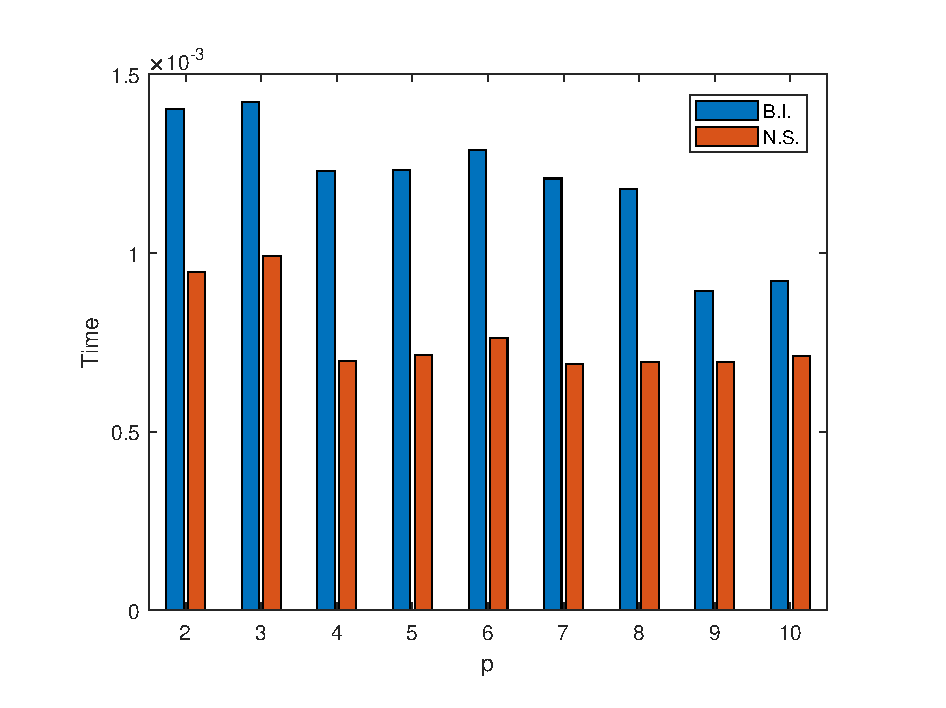
\includegraphics{n10.pdf}}
\caption{Time in example 4.1}
\end{center}
\end{figure}

\end{example}


\begin{example}
\cite{JH}Let matrix $A=rand(50)\times 10^{-2}$ ,$Q=eye(50)$ and $p=2,3, \cdots,10$.

\begin{center}
\begin{tabular}{c|c|c|c|c|c}
                       &  B.I.-iter  &  B.I.-time  &  N.S.-iter  &  N.S.-time \\ \hline\hline
$p=2$                    &  8          &  0.0177     &  8          &  0.0050  \\ \hline
$p=3$                    &  8          &  0.0173     &  6          &  0.0039  \\ \hline
$p=4$                    &  7          &  0.0146     &  7          &  0.0046  \\ \hline
$p=5$                    &  7          &  0.0147     &  7          &  0.0048  \\ \hline
$p=6$                    &  7          &  0.0149     &  7          &  0.0051  \\ \hline
$p=7$                    &  6          &  0.0128     &  7          &  0.0051  \\ \hline
$p=8$                    &  6          &  0.0128     &  7          &  0.0053  \\ \hline
$p=9$                    &  6          &  0.0133     &  7          &  0.0054  \\ \hline
$p=10$                   &  6          &  0.0132     &  6          &  0.0046  \\ \hline
\end{tabular}
\end{center}

\begin{figure}
\begin{center}
\resizebox{12cm}{8cm}{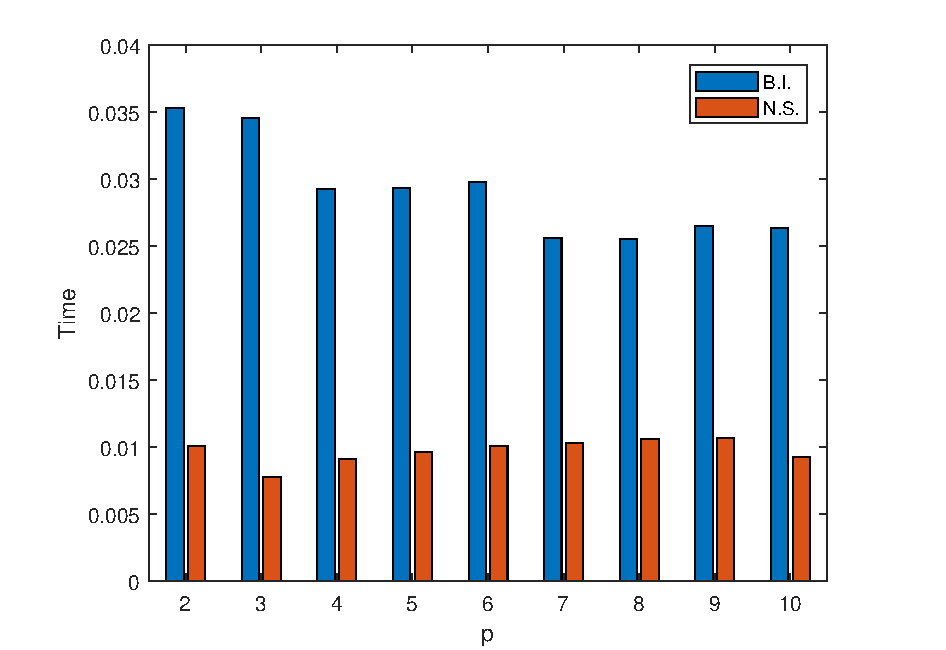
\includegraphics{n50.pdf}}
\caption{Time in example 4.2}
\end{center}
\end{figure}

\end{example}



In section 3, we showed the local convergence of the method (\ref{jie}). Now, we will calculate the convergence radius of the following examples. We used matrix 2-norm for calculation.
\begin{example}
Let $A=\left(\begin{array}{cc}
                0.5& -0.45\\
                0.45& 0
               \end{array}\right),\
               Q=\left(\begin{array}{cc}
                1 & 0\\
                0 & 1
               \end{array}\right)$, $p=2,3,4,5,6$.

\begin{center}
\begin{tabular}{c|c|c|c}
      & $s$     & $a$     & $\delta$     \\ \hline
$p=2$   & 0.6902  & 0.7648  & 0.6682       \\ \hline
$p=3$   & 0.7713  & 0.7648  & 0.6372       \\ \hline
$p=4$   & 0.8186  & 0.7648  & 0.6361       \\ \hline
$p=5$   & 0.8497  & 0.7648  & 0.6403       \\ \hline
$p=6$   & 0.8717  & 1.0215  & 0.6453       \\ \hline
\end{tabular}
\end{center}

\end{example}


\begin{example}
Let $A=\left(\begin{array}{cc}
                0.2& 0.4\\
                0.05& 0.25
               \end{array}\right),\
               Q=\left(\begin{array}{cc}
                1 & 0\\
                0 & 1
               \end{array}\right)$, $p=2,3,4,5,6$.

\begin{center}
\begin{tabular}{c|c|c|c}
      & $s$     & $a$     & $\delta$     \\ \hline
$p=2$   & 0.8716  & 0.5114  & 2.8393       \\ \hline
$p=3$   & 0.9099  & 0.5114  & 2.7818       \\ \hline
$p=4$   & 0.9306  & 0.5114  & 2.7663       \\ \hline
$p=5$   & 0.9435  & 0.5114  & 2.7632       \\ \hline
$p=6$   & 0.9524  & 0.5114  & 2.7641       \\ \hline
\end{tabular}
\end{center}

\end{example}

The iteration number of N.S. algorithm is equal to or greater than Built-in function in MATLAB when we compare only the iteration numbers. We don't check the iteration number of Built-in function when we use it to find the $p$-th root. We reduce CPU-time for finding the $p$-th root at each steps. By the N.S. algorithm, we save the CPU time to find the solution. We can consider other methods which evaluate the matrix $p$-th root. Some other methods also reduce the CPU-time. For example, we also checked the Halley method in \cite{C.H.Guo} and it also reduces CPU-time, but it is slower than N.S. algorithm. It is possible to find suitable algorithms for solving the equation (\ref{eq}) in various conditions of coefficient matrices.


\bibliographystyle{plain}
\bigskip


\begin{flushleft}
{\bf References}
\end{flushleft}

\begin{thebibliography}{10}
\bibitem{S.M.EL}{ S. M. EL-Sayed and A. C. M. Ran, On an iteration method for solving a class of nonlinear matrix equautions, SIAM J. Matrx Anal. Appl. 23 (2001) 632-645.}
\bibitem{J.C.}{ J. C. Engwerda, A. C. M. Ran and A. L. Rijkeboer, Necessary and sufficient conditions for the existence of a positive solution of the matrix equation $X+A^*X^{-1}A=Q$, Linear Algebra Appl. 186 (1993) 255-275.}
\bibitem{Jia}{ Z. Jia and M. Wei, Solvability and sensitivity theory of  polynomial matrix equation $X^s+A^TX^tA=Q$, Appl. Math. Comput. 209 (2009) 230-237.}
\bibitem{I.C.M.Ran}{ A. C. M. Ran and M. C. B. Reurings, On the nonlinear matrix equation $X+A^*{\mathscr{F}}(X)A=Q$: solution and perturbation theory, Linear Algebra Appl. 346 (2002) 15-26.}
\bibitem{JH}{ J. Meng and H.-M. Kim, The positive definite solution to a nonlinear matrix equation, Linear and Multilinear Algebra, Vol. 64, No. 4, (2016) 653-666.}
\bibitem{A.C.M3}{ A. C. M. Ran and M. C. B. Reurings, The symmetric linear matrix equation, Electron. J. Linear Algebra 9 (2002) 93-107.}
\bibitem{A.C.M2}{ A. C. M. Ran and M. C. B. Reurings, A nonlinear matrix equation connected to interpolation theory, Linear Algebra Appl. 379 (2004) 289-302.}
\bibitem{M.C.B}{ M. C. B. Reurings, Contractive maps on normed linear spaces and their applications to nonlinear matrix equations, Linear Algebra Appl. 418 (2006) 292-311.}
\bibitem{M.C.B2}{ M. C. B. Reurings, Symmetric Matrix Equations, Ph.D. thesis, Vrije Universiteit Amsterdam, 2003. $<$http://www.math.vu.nl/proefschriften/ Reurings$>$.}
\bibitem{C.H.Guo}{ C.-H. Guo, On Newton’s method and Halley’s method for the principal $p$-th root of a matrix, Linear Algebra Appl. 432 (2010) 1905-1922.}
\bibitem{N.J.Higham}{ N. J. Higham, Functions of Matrices : Theory and Computation, SIAM, Philadelphia,2008.}

\bibitem{Bini-Higham-Meini}{ D. A. Bini, N. J. Higham and B. Meini, Algorithms for the matrix $p$th root, Numer. Algorithms 39 (2005) 349-378.}
\bibitem{Guo-Higham}{ C.-H.Guo and N. J. Higham, A Schur-Newton method for the matrix $p$th root and its inverse, SIAM J. Matrix Anal. Appl. 29 (2007) 396-412.}
\bibitem{Iannazzo1}{ B. Iannazzo, On the Newton method for the matrix $p$th root, SIAM J. Matrix Anal. Appl. 28 (2006) 503-523.}
\bibitem{Iannazzo2}{ B. Iannazzo, A family of rational iterations and its applications to the computation of the matrix $p$th root, SIAM J. Matrix Anal. Appl. 30 (2008) 1445-1462.}

\bibitem{M.I.Smith}{ M. I. Smith, A Schur Algorithm for computing matrix $p$th roots, SIAM J. Matrix Anal. Appl. 24 (2003) 971-989.}
\bibitem{R.A.Smith}{ R. A. Smith, Infinite product expansions for matrix $n$-th roots, J. Austral. Math. Soc. 8 (1968) 242-249.}
\bibitem{Sadeghi}{ A. Sadeghi, A. I. Md. Ismail and A. Ahmad, Computing the $p$th Roots of a matrix with Repeated Eigenvalues, Applied Mathematical Sciences, Vol. 5, No. 53, (2011) 2645-2661.}
\bibitem{Ortega2000}{J. M. Ortega and W. C. Rheinboldt, Iterative solution of nonlinear equations in several variables, Academic Press, New York, (2000)}
\bibitem{Cheng-Higham}{ S. H. Cheng, N. J. Higham, C. S. Kenney and A. J. Laub, Approximating the logarithm of a matrix to
specified accuracy, SIAM J. Matrix Anal. Appl. 22(4) (2001) 1112-1125.}
\bibitem{Kenney-Laub}{ C. S. Kenney and A. J. Laub, Condition estimates for matrix functions, SIAM J. Matrix Anal. Appl.
10(2) (1989) 191-209.}
\bibitem{Hoskins-Walton}{ W. D. Hoskins and D. J. Walton, A faster, more stable method for computing the pth roots of positive
definite matrices, Linear Algebra Appl. 26 (1979) 139-163.}
\bibitem{Shieh-Tsay-Yates}{ L.-S. Shieh, Y. T. Tsay and R. E. Yates, Computation of the principal nth roots of complex matrices, IEEE Trans. Automat. Control 30(6) (1985) 606-608.}
\bibitem{YJ-JH}{ Y.-J. Kim, J.-H. Seo and H.-M. Kim, Local convergence of functional iterations for solving a quadratic matrix equation, accepted to B. Korean Math. Soc.}


\end{thebibliography}

\end{document}
